In this Chapter we briefly try to shed some light on the question ``what is data science?''. First of all, it is important to realize that data science is not a new concept. There are many complex definitions out there, but in our view, data science is simply the coupling of very well-established disciplines, such as mathematics and statistics, with a relatively young discipline, computer sciences. 

Have a look at Fig. \ref{fig:Analytics}. It shows the evolution of 5 fundamental disciplines related to data science (Mathematics, Statistics, visualization, technology, computer science). Note that this cartoon depicts events as old as the ``invention'' of modern calculus by Newton/Leibniz (in the 17$^{th}$ century) or foundation of probability theory by Cardano (in the 16$^{th}$ century). You can see that back in those times all the disciplines were really self-contained areas without much interconnection. As we enter the 20$^{th}$ century things start to get more interconnected. Statistics and Mathematics cannot be separated so clearly any more (e.g. stochastic models, survival models), and computer sciences and technology started to gain more terrain (e.g. relational databases, tree-based models). 
\newpage
\begin{figure}[h]
	\begin{center}
			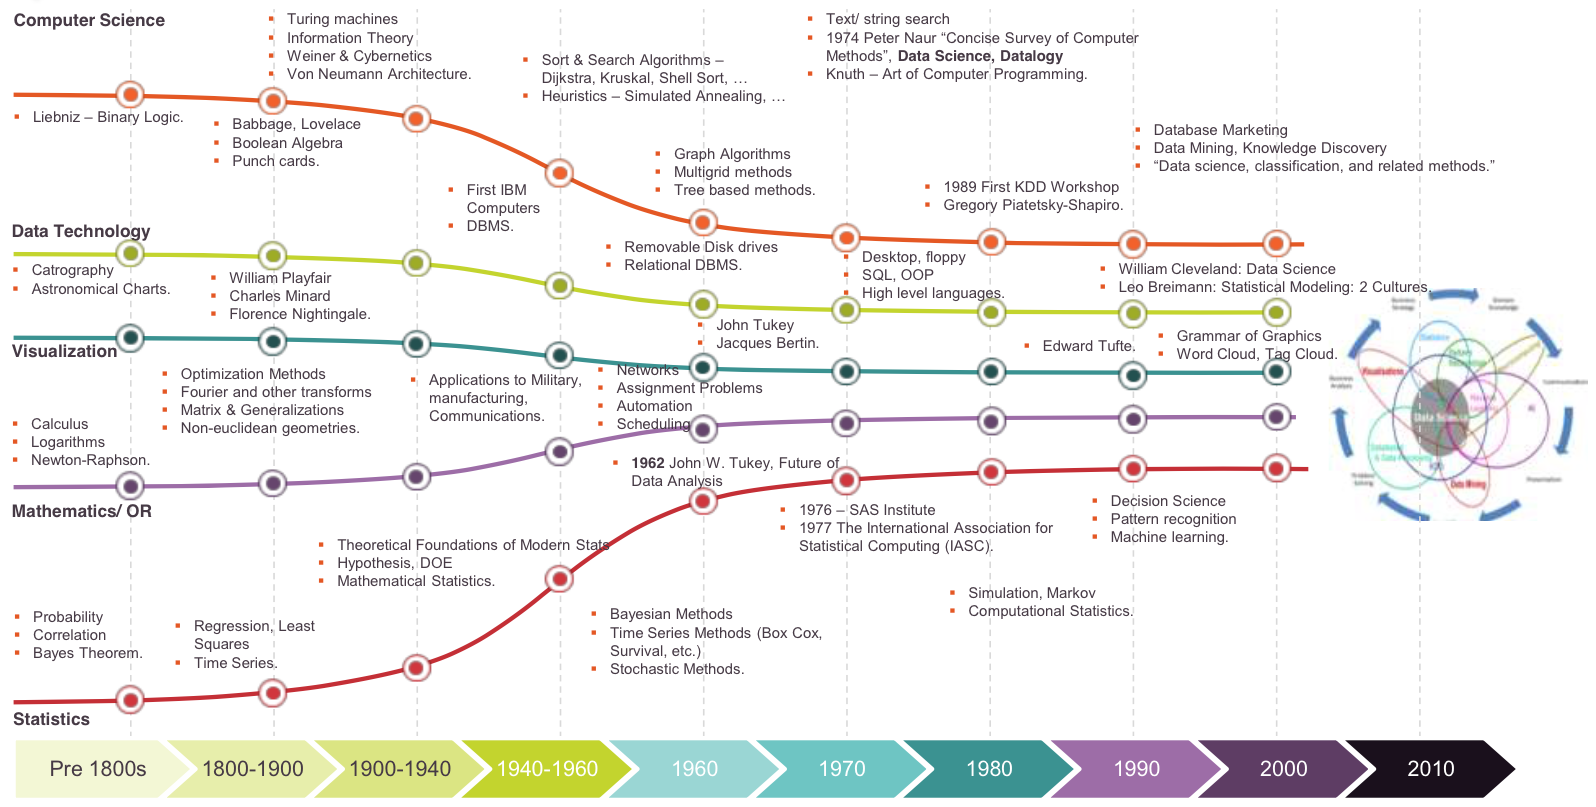
\includegraphics[scale=0.25]{Parts/history/HistoryCH1.png}
	\end{center}
	\caption{Most important events in the history of data science. \textit{Credit: Mamatha Upadhyaya}}
	\label{fig:Analytics}
\end{figure} 

As early as 1962, John Wilder Tukey, an American Mathematician, wrote in his ``The future of data'':
\begin{quotation}
\textit{For a long time I thought I was a statistician, interested in inferences from the particular to the general. But as I have watched mathematical statistics evolve, I have had cause to wonder and doubt. I have come to feel that my central interest is in data analysis. Data analysis, and the parts of statistics which adhere to it, must take on the characteristics of science rather than those of mathematics data analysis is intrinsically an empirical science.}
\end{quotation} 
 
That served as inspiration to Tukey who, in 1977, published his most well-known book ``Exploratory Data Analysis''. In that book, he argued that exploratory and confirmatory data analyses must proceed alongside. Also in the 1970's, Peter Naur, Danish computer science pioneer, published the important ``Concise Survey of Computer Methods''. In this book, the term data science was used for the first time. According to him, data science can be defined as:
\begin{quotation}
\textit{The science of dealing with data, once they have been established, while the relation of the data to what they represent is delegated to other fields and sciences.}
\end{quotation} 

In the beginning of the 21$^{st}$ century all the disciplines related to data science merged. In 2008, Jeff Hammerbacher (Facebook) and DJ Patil (LinkedIn) used the terminology ``Data scientist'' to define their work and teams. Since then, the use of this terminology has fully infiltrated the vernacular, and did not stop growing. 

Today, data science and computer sciences (through machine learning) have been put together as almost synonyms. There are new terminologies appearing every year, such as Deep Learning, Big Data, Data Mining. Today, we understand that data science and big data do not mean (just) ``lots of data''. Instead, it means the creation of a new paradigm in how we do analysis and combine the use of our traditional tools (Mathematics and Statistics) with the technology available nowadays.